% BACKGROUND
% - What technology is the project based on?
%   - Describe the concept of the FREEDM smart-grid
%   - Introduce the idea of using GM to coordinate power resources
%   - Introduce LB as the algorithm that acctually applies the transactions and migrates power
%       - Describe as a flow control algorithm
%   - RED/ECN as a network management technique
%       - RED tries to maintain an everage queue size for a packet queue in a network device.
%       - Packets arriving after the queue is at a certain threshold may be randomly dropped or flagged to signal to the sender that queue is filling
%       - This probability is governed by things.
%       - At a hard limit packets are droped at rate x.
%       - RED also has a gentle mode where the hard rate has a second probability rate up to 2X max threshold.
%       - Packets are always dropped when the queue is full
%       - Used with ECN - a technique for managing congestion. RED can also set an ECN bit in the TCP header instead of dropping.
%       - ECN is typically limited to TCP applications.
%       - Our work tries to apply it to a UDP application to show its usefulness in a CPS.
%   - DGI Theory
%       - Real-time power management
%       - One and done UDP packet transmission with algorithm design that tolerates omission failures.
%       - Load-balancing basic theory.
%       - GM basic theory.
%   - Motivate Problems further
%       - Problem 1 - Groups being unable to form prevents the smart grid from accomplishing anything. Cite previous work as examples of exploration in this area.
%       - Problem 2 - However the configuration is value because:
%           - It detects resources that are no longer reachable or may be difficult to reach
%           - We care about this because related work indicates that k messages (failed migrations) are bad
%           - Diagram a failed migration
%           - Physical networks can handle some predetermined number of k based on their characteristics before they crash

\section{Background}

\subsection{DGI}

\subsubsection{Automatic Configuration}

The DGI uses a variation on the leader election algorithm, ``Invitation Election Algorithm,'' written by Garcia-Molina\cite{INVITATIONELECTION}.
This algorithm provides a robust election procedure which allows for transient partitions.
Transient partitions are formed when a faulty link inside a group of processes causes the group to divide temporarily.
These transient partitions merge when the link becomes more reliable.

The elected leader is responsible for making work assignments, identifying and merging with other coordinators when they are found, and maintaining an up-to-date list of peers.
Group members monitor the group leader by periodically checking if the group leader is still alive by sending a message.
If the leader fails to respond, the querying peers will enter a recovery state and operate alone until they can identify another coordinator.
Therefore, a leader and each of the members maintain a set of currently reachable processes, a subset of all known processes in the system.

Using a leader election algorithm allows the FREEDM system to autonomously reconfigure rapidly in the event of a failure.
Cyber-components are tightly coupled with the physical components, and reaction to faults is not limited to faults originating in the cyber domain.
Processes automatically react to crash-stop failures, network issues, and power system faults.
The automatic reconfiguration allows processes to react immediately to issues, faster than a human operator, without relying on a central configuration point.
However, it is important the configuration a leader election supplies is one where the system can do viable work without causing physical faults like voltage collapse or blackouts\cite{HARINI}.

A state machine for the election portion of the election algorithm is shown in Figure \ref{fig:statemachine}.
In the normal state, the election algorithm regularly searches for other coordinators to join with.
When another coordinator is identified, all other processes will yield to their future coordinator.
The method of selecting which process becomes the coordinator of the new group differentiates the modified algorithm from other approaches.

Proceses determine the optimal coordinator (the one with the lowest process ID) through the exchange of ``Are You There'' and ``Are You Coordinator'' messages.
Processes will only accept an invites from processes which are more optimal than itself, and more optimal than its current leader.
Once a timeout expires, the coordinator will send a ``Ready'' message with a list of peers to all processes that accepted the invite.
To prevent live-lock the process does not leave its previous group until the new Ready message arrives, unlike the original ``Invitation Election Algorithm''.
The invited processes have timeouts for when they expect the ready message to arrive.

\begin{figure*}[!t]
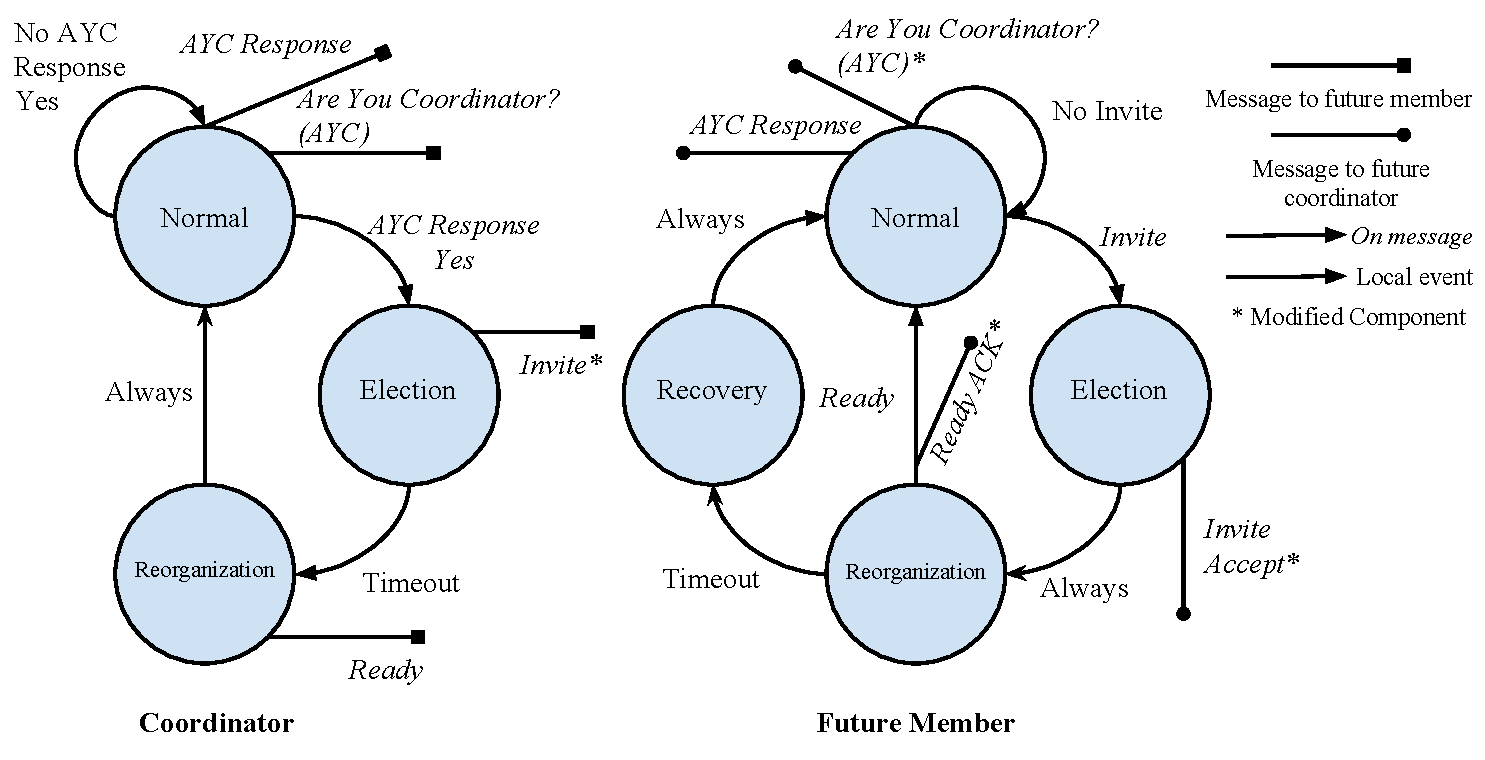
\includegraphics[width=\linewidth]{LeaderElectionStateDiagram2.pdf}
\caption{State machine of a leader election. Processes start as coordinators in the ``Normal'' state and search for other coordinators to join with. Processes immediately respond to ``Are You Coordinator'' (AYC) messages they receive. The algorithm was modified by adding a ``Ready Acknowledgment'' message as the final step of completing the election. Additionally, processes only accept invites if they have received an ``AYC Response'' message from the inviting process.}
\label{fig:statemachine}
\end{figure*}

Once a group is formed it must be maintained.
To do this, processes occasionally exchange messages to verify the other is still reachable.
This interaction is shown in Figure \ref{fig:statemachine2}.
Coordinators send ``Are You Coordinator'' messages to members of its group to check if the process has left the group.
Group members send ``Are You There'' messages to the coordinator to verify they haven't been removed from the group, and to ensure the coordinator is still alive.
If processes fail to reply to received message before a timeout, they will leave the group.
Leaving the group can either be caused by the coordinator removing the process, or the process can enter a recovery state and leave the group, forming a new group by itself.

\begin{figure*}[!t]
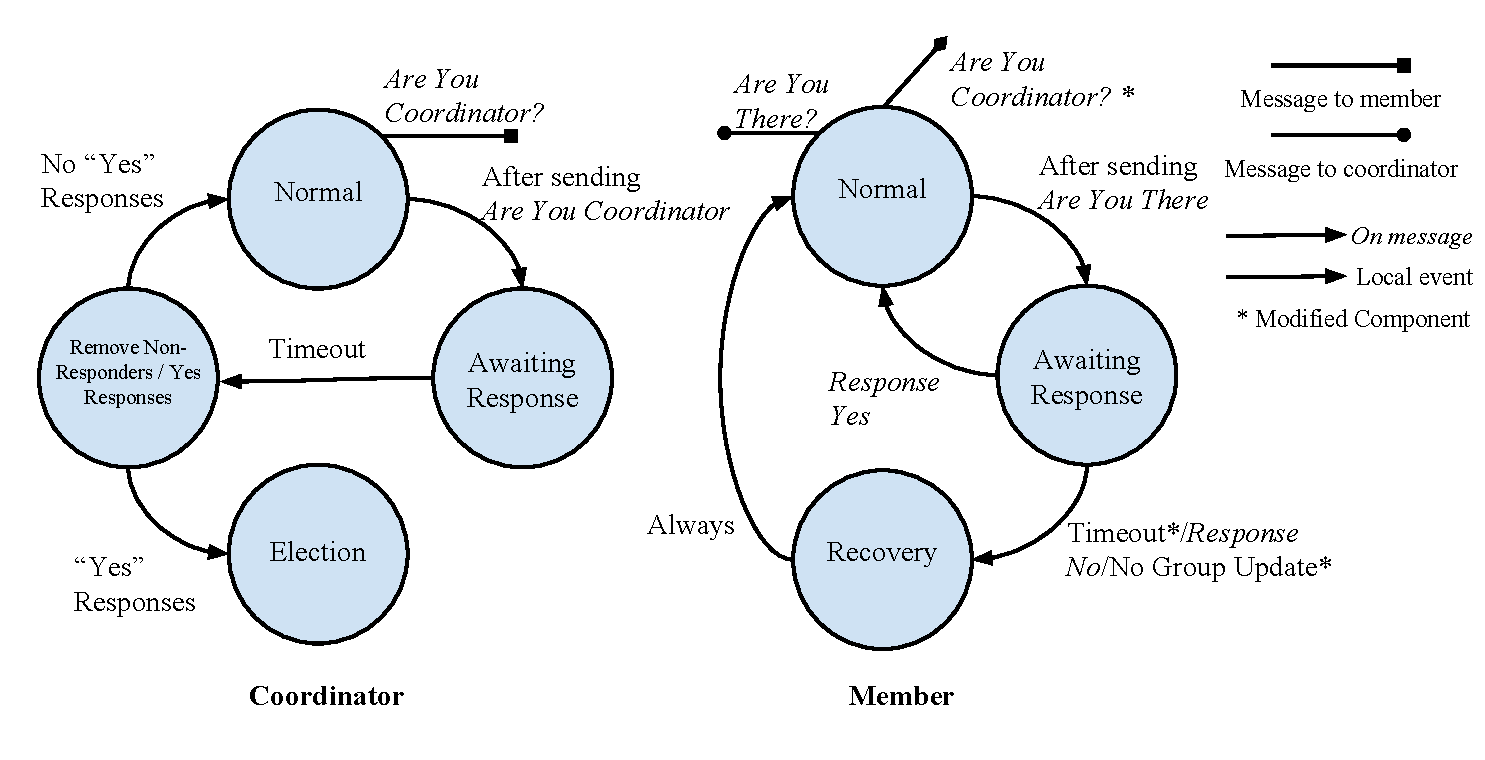
\includegraphics[width=\linewidth]{MaintainStateDiagram2.pdf}
\caption{State machine of maintaining a group. The ``Are You Coordinator'' (AYC) messages are the same as those in Figure \ref{fig:statemachine}. AYC and ``Are You There'' (AYT) are periodically sent by processes, and responses to those messages are immediately sent by the receiving process. In the modified algorithm, the member does not enter the recovery state if they do not receive an AYT response before the timeout expires.}
\label{fig:statemachine2}
\end{figure*}

This modifed algorithm allows the interactions of the processes in our semi-synchronous system to be modelable with a Markov chain.
A version of this algorithm with restriction on what processes could be come coordinator is presented in JOURNAL.
This version also removes the potential live-lock due to crash failure, although crash-failure is not considered in this work.
We elected to use an improved version of the algorithm in this work because of its easy to follow group state.
Other algorithms could be more efficent and less bursty during normal operation, however they are more inconsistent during network congestion and omission.

\subsubsection{Power Management}

In this work we utilize the load balancing algorithm from CITE RAVI.
The load balancing algorithm manages power resources by using a sequence of migrations.
In each migration, a sequence of message exchanges identify processes whose power resources are not sufficient to meet their local demand and other processes supply them with power by utilizing a shared bus.
To do this, first processes that cannot meet their demand announce their need to all other processes.
Processes with resources that exceed their demand offer their power to processes that announced their need.
The processes perform a three-way handshake.
At the end of the handshake, the two processes have issued commands to their attached resources to supply power from the shared bus and to draw power from the shared bus.

The DGI executes these modules using a round-robin real-time schedule.
Processes synchronize their clocks and execute modules semi-synchronously.
Each time the load balancing module is scheduled to execute it performs multiple migrations during it's execution phase.
This schedule is depicted in Figure \ref{fig:normal-schedule}.
In the figure, each time the load balancing module runs it has the opportunity to complete a fixed number of migrations during its execution window.
The schedule for the DGI is decided before the process is started and does not change when the DGI is running.
All DGI processes that can potentially group together use the same schedule.

\begin{figure}
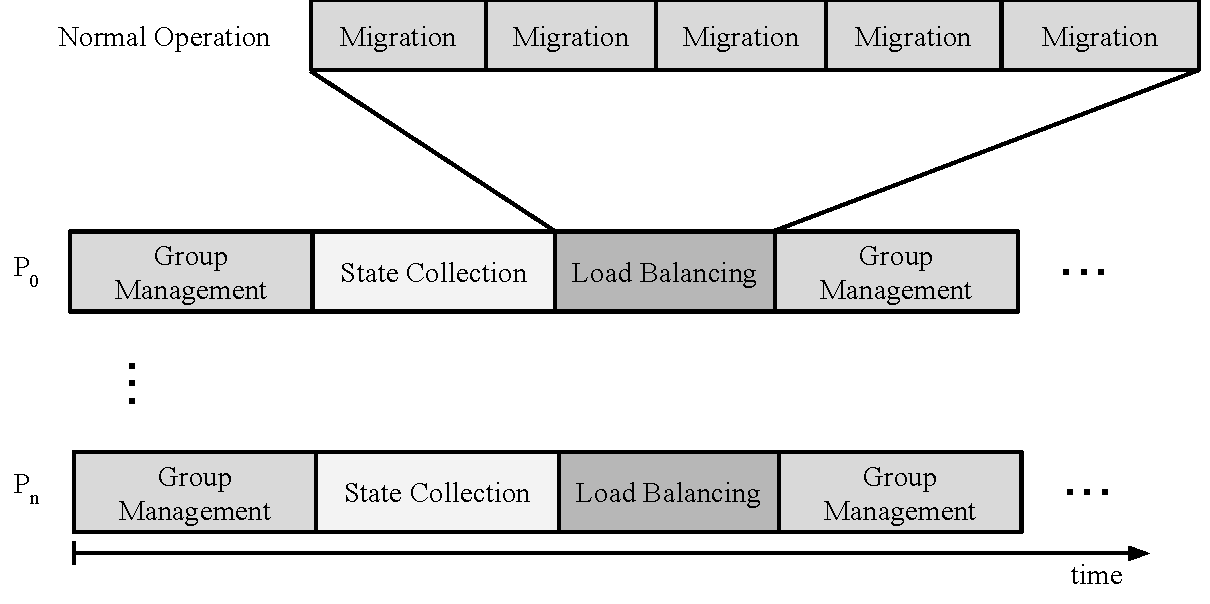
\includegraphics[width=\linewidth]{NormalDGISchedule}
\caption{Example of DGI schedule. Processes attempt a fixed number of migrations each round.} \label{fig:normal-schedule}
\end{figure}

The DGI algorithms can tolerate packet loss and is implemented using UDP to pass messages between DGI processes.
Effects of packet loss on the DGI's group management module have been explored in CRITIS and JOURNAL.
The load balancing algorithm can tolerate some message loss, but lost messages can cause migrations to only partially complete, which can cause instability in the physical network.
A failed migration is diagrammed in Figures \ref{fig:failed-migration-1} \ref{fig:failed-migration-2}.

\begin{figure}
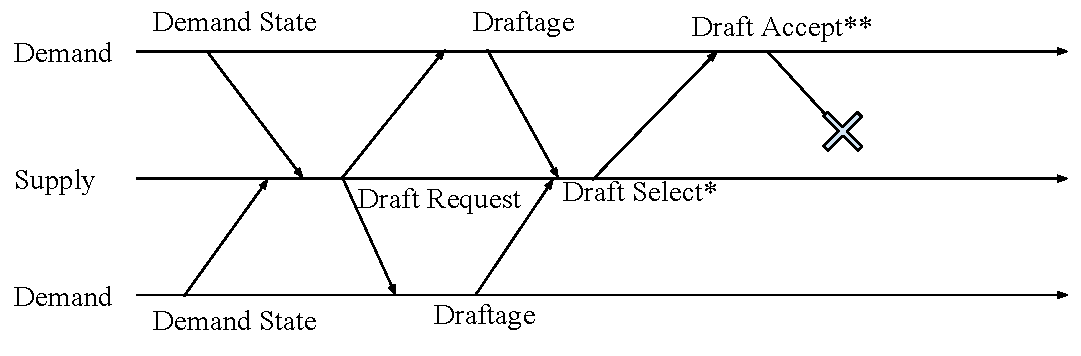
\includegraphics[width=\linewidth]{FailedMigration1}
\caption{Example of a failed migration. (*) and (**) mark moments when power devices change state to complete the physical component of the migration. In this scenario, the message confirming the demand side made the physical is lost, leaving the supply node uncertain.} \label{fig:failed-migration-1}
\end{figure}

\begin{figure}
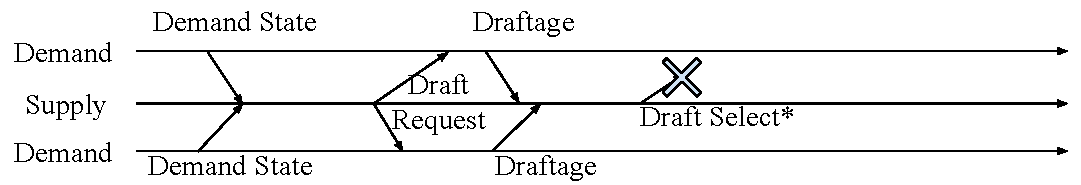
\includegraphics[width=\linewidth]{FailedMigration2}
\caption{Example of a failed migration. (*) marks a moment when power devices change state to complete the physical component of the migration. In this scenario, the supply process changes its device state, but the demand process does not.} \label{fig:failed-migration-1}
\end{figure}

With this power migration algorithm, uncompensated actions may occur in the power system.
This actions can eventually lead to power instability through issues such as voltage collapse.
Additionally, the supply process may not always be certain if the second half of the action was completed or not.
If the ``Draft Accept'' message does not arrive from the demand process, the supply process cannot be certain of wether or not its ``Draft Select'' message was received.
If the supply process takes action to compensate by reversing the migration and the confirmation arrives later the system will also be driven towards instability because another process completed an uncompensated action.
Processes could potentially confirm the number of failed migrations with a state collection technique.

It is therefore diserable to manage the processes to minimize the number failed migrations that occur.
In this work, we consider effects due to delays by congestion.
A real-time system implementing this algorithm could count the number of failed migrations with a counter.
The counter will increase when the physical side makes a change, increasing the number of outstanding migrations.
The demand process will make their physical change and send the draft accept message.
On receipt, the counter is reduced by one.
A real-time deadline is enforced on the receipt of the Draft Accept-- if the message does not arrive before a specific time interval, the counter will not be decreased.

\subsection{Random Early Detection}
The RED queueing algorithm is a popular queueing algorithm for network devices.
It uses a probabilistic model and an exponentially weighted moving average (EWMA) to determine if the average queue size exceeds predefined values.
These values are used to identify potential congestion and manage it.
This is accomplished by determining the average size of the queue, and then probabilistically dropping packets to maintain the size of the queue.
In RED, when the average queue size $avg$ exceeds a minimum threshold ($min_{th})$), but is less than a maximum threshold ($max_{th}$), new packets arriving at the queue may be ``marked''.
The probability that a packet is marked is based on the following relation between $p_{b}$ and $p_{a}$ where $p_{a}$ is the final probability a packet will be marked.

\begin{equation}
p_{b} = max_p (avg - min_{th}) / (max_{th}-min_{th})
\end{equation}
\begin{equation}
p_{a} = p_{b} / (1-count * p_b)
\end{equation}

Where $max_p$ is the maximum probability that a packet will be marked when the queue size is between $min_{th}$ and $max_{th}$ and $count$ is the number of packets since the last marked packet.
With this approach, $p_{b}$ varies linearly with the average queue size, and the $p_{a}$ is a function of that probability and the time since the last packet was marked.
If $avg$ is greater than $max_{th}$, in the gentle variation of the algorithm, the probability of marking increases from $max_p$ to 1 as the average queue size approaches $2*max_{th}$
In this work, we follow the recommendation of the authors and use the gentle variation.
In the event that the queue fills completely, the RED queue operates as a drop-tail queue.

In a simple implementation of the RED algorithm, marked packets are dropped.
For a TCP application, the result of the dropped packets causes the slow-start congestion control strategy to reduce the rate that packets are sent.
A more advanced implementation, using ECN, sets specific bits in the TCP header to indicate congestion.
By using ECN, TCP connections can reduce their transmission rate without re-transmitting packets.

UDP applications have not typically utilized ECN.
Although the ECN standard has flags in the IPv4 header, access to the IPv4 header is not possible on most systems, most notably linux.
Furthermore, there is not a "one size fits all" solution to congestion in UDP algorithms.
However, for the DGI and a class of similiar real-time processes, congestion notification has great potential.
If processes can adjust the amount of traffic they send based on the anticipated congestion (by disabling features, for example), they can decrease the effects of that congestion.

